% point_encadrant_schemas.tex
% =====================================================================
% Les schemas TikZ de `point_encadrant.tex`, et le fil d'Ariane.
%
% POURQUOI UN FICHIER SEPARE
%   `verif_chiffres_tex.py` extrait tout litteral numerique du .tex et le
%   cherche dans les Parquet. Les coordonnees TikZ en seraient ramassees
%   comme des mesures introuvables. Les schemas vivent donc ici, et le
%   controle de tracabilite porte sur `point_encadrant.tex` seul -- ou
%   chaque chiffre est bien une mesure.
%
%   Corollaire : AUCUN chiffre de mesure ne doit entrer dans ce fichier.
%   Les quatre schemas sont STYLISES, SANS DONNEES, comme les trois
%   schemas du pitch, et chaque legende le dit a l'ecran.
% =====================================================================

\usetikzlibrary{positioning, arrows.meta, patterns, decorations.pathreplacing}

% --- Palette : lisible en N&B comme le veut la regle de redaction ------
\definecolor{ctranche}{gray}{0.28}
\definecolor{couvert}{gray}{0.62}
\definecolor{cfond}{gray}{0.93}

% ---------------------------------------------------------------------
% Fil d'Ariane : les cinq pastilles, celle en cours en gras.
% L'argument est le RANG de la pastille active (1 = A ... 5 = lambda),
% pas son nom : comparer des chaines demanderait \pdfstrcmp, dont le nom
% n'est pas stable entre pdftex et luatex.
% Usage : \fildariane{3}   % met C en gras
% ---------------------------------------------------------------------
\newcommand{\fildariane}[1]{%
  \begin{tikzpicture}[baseline=-2pt]
    \foreach \q [count=\i] in {A,B,C,D,{$\lambda$}} {
      \pgfmathsetmacro{\x}{(\i-1)*1.0}
      \ifnum\i=#1
        \node[draw=ctranche, fill=ctranche, text=white, rounded corners=2pt,
              minimum width=0.72cm, minimum height=0.30cm,
              font=\bfseries\scriptsize] at (\x,0) {\q};
      \else
        \node[draw=couvert, text=couvert, rounded corners=2pt,
              minimum width=0.72cm, minimum height=0.30cm,
              font=\scriptsize] at (\x,0) {\q};
      \fi
    }
  \end{tikzpicture}%
}

% ---------------------------------------------------------------------
% Schema 1 -- la carte des questions (slide 2)
% ---------------------------------------------------------------------
\newcommand{\schemaCarte}{%
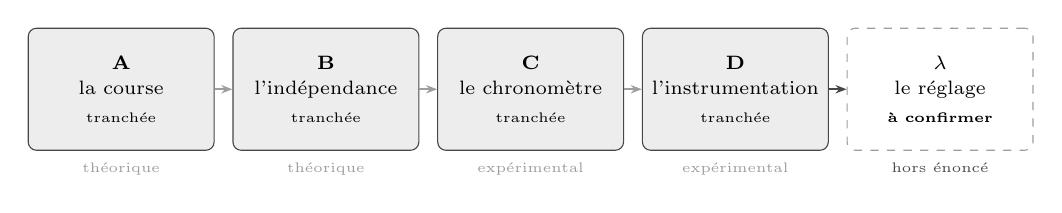
\begin{tikzpicture}[
    q/.style={draw=ctranche, fill=cfond, rounded corners=3pt,
              text width=2.15cm, minimum height=1.55cm, align=center,
              font=\scriptsize, inner sep=3pt},
    ouvert/.style={q, draw=couvert, dashed, fill=white},
    lien/.style={-{Stealth[length=4pt]}, couvert, thick}]

  \node[q] (a) at (0,0)
    {\textbf{A}\\[1pt]\scriptsize la course\\[2pt]\tiny tranchée};
  \node[q] (b) at (2.6,0)
    {\textbf{B}\\[1pt]\scriptsize l'indépendance\\[2pt]\tiny tranchée};
  \node[q] (c) at (5.2,0)
    {\textbf{C}\\[1pt]\scriptsize le chronomètre\\[2pt]\tiny tranchée};
  \node[q] (d) at (7.8,0)
    {\textbf{D}\\[1pt]\scriptsize l'instrumentation\\[2pt]\tiny tranchée};
  \node[ouvert] (l) at (10.4,0)
    {$\boldsymbol\lambda$\\[1pt]\scriptsize le réglage\\[2pt]\tiny \textbf{à confirmer}};

  \draw[lien] (a) -- (b);
  \draw[lien] (b) -- (c);
  \draw[lien] (c) -- (d);
  \draw[lien, ctranche] (d) -- (l);

  \node[couvert, font=\tiny, below=1pt of a] {théorique};
  \node[couvert, font=\tiny, below=1pt of b] {théorique};
  \node[couvert, font=\tiny, below=1pt of c] {expérimental};
  \node[couvert, font=\tiny, below=1pt of d] {expérimental};
  \node[ctranche, font=\tiny, below=1pt of l] {hors énoncé};
\end{tikzpicture}%
}

% ---------------------------------------------------------------------
% Schema 2 -- les deux CDF (slide 5, question B)
% L'axe ne porte AUCUNE graduation chiffree : la forme seule est le propos.
% ---------------------------------------------------------------------
\newcommand{\schemaCDF}{%
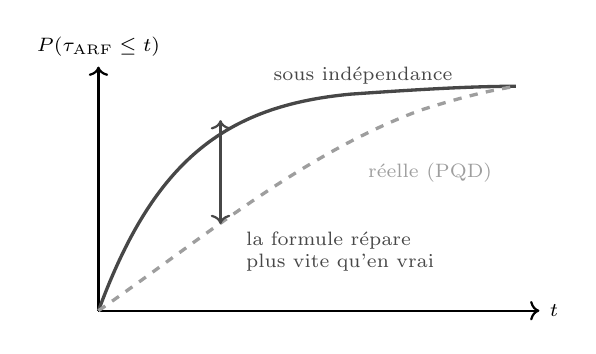
\begin{tikzpicture}[scale=1]
  \draw[->, thick] (0,0) -- (5.6,0) node[right, font=\scriptsize] {$t$};
  \draw[->, thick] (0,0) -- (0,3.1)
       node[above, font=\scriptsize] {$P(\tau_{\mathrm{ARF}} \le t)$};

  % CDF sous independance : monte plus vite (reparation "trop rapide")
  \draw[ctranche, very thick]
    (0,0) .. controls (0.7,1.9) and (1.6,2.6) .. (3.2,2.75)
          .. controls (4.2,2.82) and (4.8,2.85) .. (5.3,2.85);
  % CDF reelle sous PQD : au-dessous partout
  \draw[couvert, very thick, dashed]
    (0,0) .. controls (1.3,0.9) and (2.6,2.0) .. (4.1,2.55)
          .. controls (4.7,2.74) and (5.0,2.80) .. (5.3,2.85);

  \node[ctranche, font=\scriptsize, anchor=west] at (2.1,2.98)
       {sous indépendance};
  \node[couvert, font=\scriptsize, anchor=west] at (3.3,1.75)
       {réelle (PQD)};

  \draw[<->, ctranche, thick] (1.55,1.10) -- (1.55,2.42);
  \node[ctranche, font=\scriptsize, anchor=west, align=left] at (1.75,0.75)
       {la formule répare\\plus vite qu'en vrai};
\end{tikzpicture}%
}

% ---------------------------------------------------------------------
% Schema 3 -- detecter n'est pas gagner (slide 8)
% Deux frises. Aucune date n'est graduee : c'est l'ordre qui est le propos.
% ---------------------------------------------------------------------
% Compact : les deux frises l'une sous l'autre, verdict EN TITRE de chaque
% frise et non a sa droite -- a droite il chevauchait la colonne de texte.
\newcommand{\schemaZombie}{%
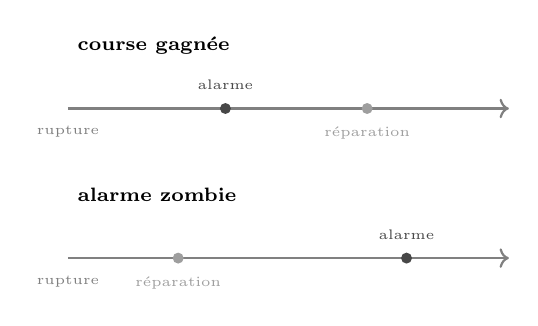
\begin{tikzpicture}[
    frise/.style={->, thick, gray},
    ev/.style={circle, fill, inner sep=1.4pt},
    et/.style={font=\tiny, align=center}]

  % --- cas gagne ---
  \node[font=\scriptsize\bfseries, anchor=west] at (0,2.45) {course gagnée};
  \draw[frise] (0,1.65) -- (5.6,1.65);
  \node[ev, ctranche] (d1) at (2.0,1.65) {};
  \node[ev, couvert]  (a1) at (3.8,1.65) {};
  \node[et, ctranche, above=1pt of d1] {alarme};
  \node[et, couvert,  below=1pt of a1] {réparation};
  \node[et, gray, anchor=north] at (0,1.55) {rupture};

  % --- cas zombie ---
  \node[font=\scriptsize\bfseries, anchor=west] at (0,0.55) {alarme zombie};
  \draw[frise] (0,-0.25) -- (5.6,-0.25);
  \node[ev, couvert]  (a2) at (1.4,-0.25) {};
  \node[ev, ctranche] (d2) at (4.3,-0.25) {};
  \node[et, couvert,  below=1pt of a2] {réparation};
  \node[et, ctranche, above=1pt of d2] {alarme};
  \node[et, gray, anchor=north] at (0,-0.35) {rupture};
\end{tikzpicture}%
}

% ---------------------------------------------------------------------
% Schema 4 -- la fenetre de A (slide 10)
% Trajectoire STYLISEE. Le propos : l'aire change de signe apres la
% transition, et H la somme jusqu'au bout.
% ---------------------------------------------------------------------
\newcommand{\schemaAire}{%
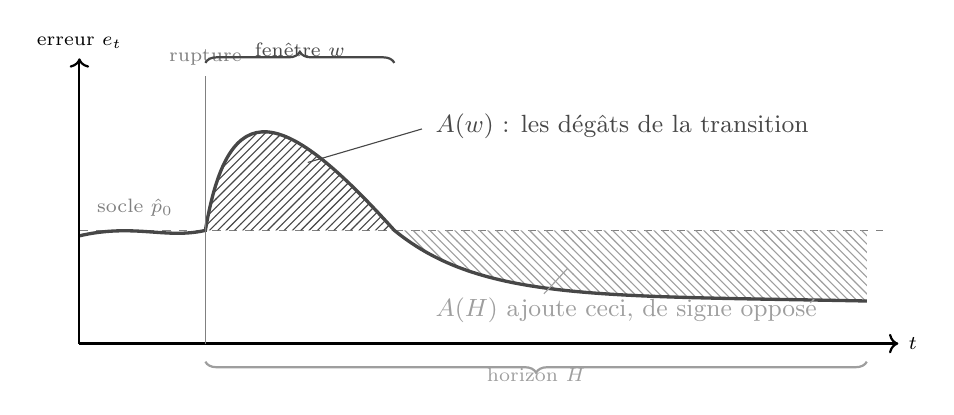
\begin{tikzpicture}[x=1cm, y=1.15cm]
  % --- socle p0, trace en premier pour passer sous les hachures --------
  \draw[gray, dashed] (0,1.6) -- (10.2,1.6);
  \node[gray, font=\scriptsize, anchor=south west] at (0.1,1.65)
       {socle $\hat p_0$};

  % --- aire positive, sur la fenetre de transition ---------------------
  \fill[pattern=north east lines, pattern color=ctranche]
    (1.6,1.6) .. controls (1.9,3.15) and (2.6,2.95) .. (4.0,1.6) -- cycle;
  % --- aire negative, tout le reste de l'horizon -----------------------
  \fill[pattern=north west lines, pattern color=couvert]
    (4.0,1.6) .. controls (5.1,0.82) and (6.6,0.88) .. (10.0,0.82)
    -- (10.0,1.6) -- cycle;

  % --- trajectoire ------------------------------------------------------
  \draw[ctranche, very thick]
    (0,1.54) .. controls (0.7,1.68) and (1.1,1.50) .. (1.6,1.6)
             .. controls (1.9,3.15) and (2.6,2.95) .. (4.0,1.6)
             .. controls (5.1,0.82) and (6.6,0.88) .. (10.0,0.82);

  % --- axes -------------------------------------------------------------
  \draw[->, thick] (0,0.35) -- (10.4,0.35) node[right, font=\scriptsize] {$t$};
  \draw[->, thick] (0,0.35) -- (0,3.5)
       node[above, font=\scriptsize] {erreur $e_t$};

  % --- rupture ----------------------------------------------------------
  \draw[gray, thin] (1.6,0.35) -- (1.6,3.3);
  \node[gray, font=\scriptsize, anchor=south] at (1.6,3.32) {rupture};

  % --- accolades --------------------------------------------------------
  \draw[decorate, decoration={brace, amplitude=4pt}, ctranche, thick]
    (1.6,3.45) -- (4.0,3.45)
    node[midway, above, font=\scriptsize, inner sep=2pt] {fenêtre $w$};
  \draw[decorate, decoration={brace, amplitude=4pt, mirror}, couvert, thick]
    (1.6,0.15) -- (10.0,0.15)
    node[midway, below, font=\scriptsize, inner sep=2pt] {horizon $H$};

  % --- legendes des deux aires, hors des hachures -----------------------
  \node[ctranche, font=\small, anchor=west] at (4.4,2.75)
       {$A(w)$ : les dégâts de la transition};
  \draw[ctranche, thin] (4.35,2.72) -- (2.9,2.35);

  \node[couvert, font=\small, anchor=west] at (4.4,0.72)
       {$A(H)$ ajoute ceci, de signe opposé};
  \draw[couvert, thin] (5.9,0.9) -- (6.2,1.18);
\end{tikzpicture}%
}
